\documentclass[a4paper, 11pt]{report}
\usepackage{graphicx}
\usepackage{xspace}
\usepackage[margin= 1in,includefoot]{geometry}
\newcommand\nth{\textsuperscript{th}\xspace}
\usepackage{xcolor}
\usepackage{lipsum}
\usepackage{listings}
\usepackage{amssymb} %maths
\usepackage{amsmath} %maths
\usepackage{mathptmx}
\begin{document}
\begin{figure}

\includegraphics[scale=.63]{medipol.png}
\centering
\end{figure}
\begin{titlepage}
\title{Introduction to Computer Engineering \\ Fall 2021, Assignment 5}
\author{by 64160010 - Rumeysa ÇELİK, Istanbul Medipol University}
\date{Due on Saturday December $25^{th}$, 2021 by 11:59 PM}
\maketitle
\end{titlepage}
{\center{\section*{{\textbf{Parameters Specific To Your Submission}}}}}
{\setlength{\parindent}{0pt}{In this assignment we will use the digits from your IDs. We define the following numbers
which are the \textbf{same} as the \textbf{numbers} you used in your assignment :}
\\ \\
$c_1$: The average of of digits from your student ID, \textbf{rounded} + 1. Use Excel file provided
to determine $c_1$.
\\ \\ My student ID is: 64160010
\begin{align*}
Average : \frac{6+4+1+6+0+0+1+0}{8} = \frac{18}{8} = 2.25 \approx 2 \\
c_1 = 2
\end{align*}
\\
$c_2$ : The average of digits from your Turkish ID, \textbf{rounded} + 1. Use the Excel file to determine $c_2$.
\\ \\
My Turkish ID is: 33098186424
\begin{align*}
Average: \frac{3+3+0+9+8+1+8+6+4+2+4}{11} = \frac{48}{11} = 4.36363636 \approx 4 \\
c_2 = 4
\end{align*}
\\
$c_3$: If $(c_1 \geq c_2)$ then $c_3 = 1$ otherwise $c_3 = -1$ .
\\ \\
$c_1 < c_2$ so that by $c_3 = -1$.
\\ \\
$c_4$ = $c_1$ + $c_2$.
\\ \\
Then,
\begin{align*}
c_4 = 2 + 4 = 6\\
c_4 = 6
\end{align*}
\\
$c_5$ : The first digit for your student ID.
\\ \\
My Student ID is: 64160010
\\ So that by $c_5$ = 6
\newpage
\section*{\textbf{Question1 (40 points):}}

Sample space is the set formed by all possible outcomes for an event. Find the sample spaces
and the size (element number) of the sample space for the given tasks.
\begin{enumerate}
\item[(a)] (10 pts.) Assume we roll round ((c5=6)/2)=3 amount of distinct fair coins once. (In this case,
the sample space is formed by head/tail combinations.)
{\color{blue}{
\begin{align*}
S=\lbrace (HHH),(TTT),(HHT),(THH),(HTH),(TTH),(THT),(HTT)\rbrace
\end{align*}}}
\item[(b)] (10 pts.) Assume we toss round(c5/2) amount of non-fair coins once and record the absolute difference between number of heads and number of tails. (In this case, the sample space formed by recorded numbers.)
\begin{figure}[h]
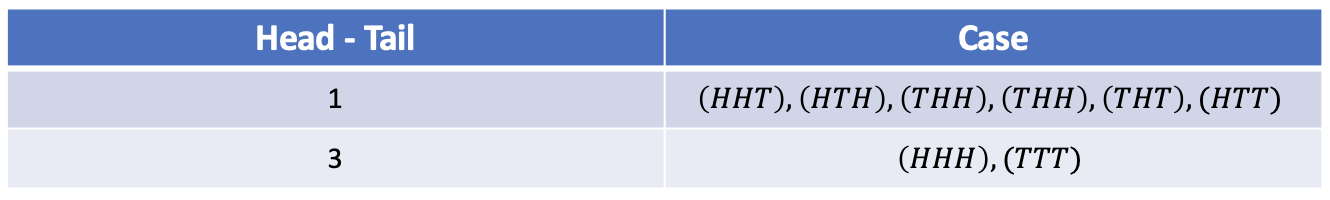
\includegraphics[scale=.57]{1.png}
\centering
\caption{{\color{blue}{$S=\lbrace 1,3 \rbrace$}}}
\end{figure}
\item[(c)] (10 pts.) Assume you have 2 distinct shirts and 4 distinct pants. You are forming outfits by combining pants with the shirts. (In this case, the sample space is formed by obtained pants-shirt combinations.) \\ \\
{\color{blue}{2 distinct shirts = R and A \\ 4 distinct pants = M, D, H, E
\begin{align*}
S = \lbrace (RH), (RM), (RE), (RD), (AH), (AM), (AE), (AD) \rbrace
\end{align*}}}
\item[(d)] (10 pts.) Assume we have a non-fair coin. We toss the coin until we obtain two successive tails. (In this case, the sample space is formed by all possible outcomes (head/tail combinations) until we reach two successive tails.)
{\color{blue}{
\begin{align*}
S = \lbrace (TT), (HTT), (HHTT), (HTHTT), (THTHTT), (HHHTT), ... , (THHTT) \rbrace
\end{align*}}}
\end{enumerate}
\newpage
\section*{\textbf{Question2 (20 points):}}

A gambling game is played by a ticket. In this game, a player will have four possibilities that he will earn or lose some dollars in return. The outcomes with the probabilities and the associated returns are given in the following chart:
\begin{figure}[h]
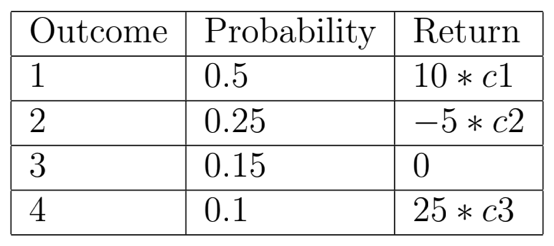
\includegraphics[scale=.57]{2.png}
\centering
\end{figure}
\\
How much would a risk-neutral person pay to play this game?
\begin{align*}
Expected \quad Value, \quad \mu = \Sigma X \cdot P(X)
\end{align*}
\begin{figure}[h]
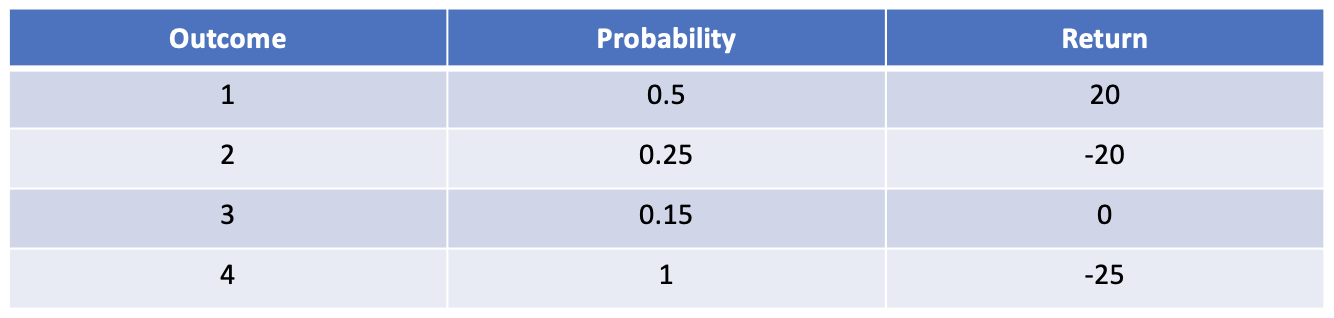
\includegraphics[scale=.57]{3.png}
\centering
\caption{{\color{blue}{$\mu = (20 \times 0.5) + (-20 \times 0.25) + (0 \times 0.15) + (-25 \times 1) = -30$}}}
\end{figure}

\newpage
\section*{\textbf{Question3 (40 points):}}

A car is on a road where there are four equally likely possible moves as going straight, turning right, turning left and stopping. There are three traffic signs in two different colors. The stop sign is in blue, left turn and right turn signs are in red. The probability of seeing a left turn sign is 1/2, probability of seeing a right turn sign is 1/4, and probability of seeing a stop sign is 1/4. For a specific traffic sign, the car moves correctly with probability 14/100 and all the incorrect moves are equally likely. Answer the following questions
\begin{figure}[h]
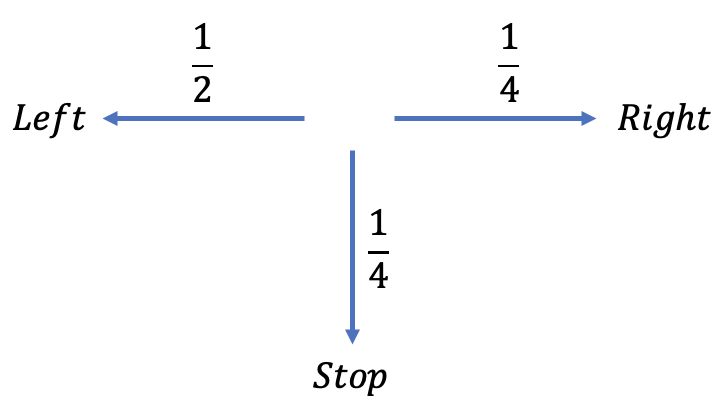
\includegraphics[scale=.57]{4.png}
\centering
\end{figure}
\begin{enumerate}
\item[(a)] (10 pts.) What is the probability that the car goes straight?
{\color{blue}{\begin{align*}
For \quad left, \qquad \frac{1}{2} \times (1 - \frac{14}{100}) \times \frac{1}{3} \\
= \frac{1}{6} \times \frac{86}{100} = \frac{86}{600} \\ 
For \quad stop \qquad \frac{1}{4} \times (1 - \frac{14}{100}) \times \frac{1}{3} \\
= \frac{1}{12} \times \frac{86}{100} = \frac{86}{1200} \\
For \quad right \qquad same \quad calculation \quad with \quad stop \quad = \quad \frac{86}{1200} \\
Total \quad probability \quad = \quad (\frac{1}{6} + \frac{1}{12} + \frac{1}{12})\cdot (\frac{86}{100}) = 0.28666667
\end{align*}}}
\item[(b)] (10 pts.) What is the probability that the car sees a red sign?
{\color{blue}{\begin{align*}
P = \frac{1}{2} + \frac{1}{4} = \frac{3}{4}\\ = 0.75
\end{align*}}}
\item[(c)] (20 pts.) What is the probability that the car turn left if it is given that it is a red sign?
{\color{blue}{\begin{align*}
\frac{2}{3} \times \frac{14}{100} = \frac{28}{100} \\
\frac{1}{3} \times (1-\frac{14}{100}) \times \frac{1}{3} \\
= \frac{1}{9} \times \frac{86}{100} = \frac{86}{900} \\
= \frac{28}{300} + \frac{86}{900} = 0.18888889
\end{align*}}}
\end{enumerate}






































\end{document}
